\section{Topology Optimisation}
\label{sec:TopOpt}
\emph{Topology optimization} describes the process of finding the optimal distribution of a limited amount of material for a given area or volume based on a predefined constraint/minimization problem. Possible optimization goals are for example \cite{Hunter2009}:
\begin{itemize}
\item \textbf{Minimum compliance}, in which one seeks to find the optimal distribution of material that returns the stiffest possible structure. The structure is thereby subjected to loads (forces) and supports (boundary conditions). By maximizing the stiffness, the compliance is minimized. This is also analogous to minimizing the stress energy stored by the applied loads.
\item \textbf{Heat conduction}, where one tries to optimize the domain of a conductive material with respect to conductivity for the purpose of heat transfer. This maximization problem is the same as minimizing the temperature gradient over the domain --- a poor conductor will create a large gradient.
\item \textbf{Mechanism synthesis}, where the objective is to obtain a device that can convert an input displacement in one location to an output displacement in another location. Thus, one hereby seeks the optimal design which maximizes the output force for a given input, or respectively, minimizes the input force for a given output.
\end{itemize}


As one can already imagine by this short list of optimization goals, topology optimization has a wide field of possible applications. Hence, it has become a well established technology used by engineers in the fields of aeronautics, civil, materials, mechanical and structural optimization. Furthermore, due to the rising significance of additive manufacturing techniques in industry, the realisation of complex optimized designs is now much easier \cite{Yang1995}.
For the rest of this section, and the rest of the document, we will concentrate on the \emph{Minimum compliance} problem. Note however, that almost all parts in the \emph{CAD-Integrated Topology Optimization} tool could just as well be applied to any other topology optimization problem. 

\subsection{Minimum Compliance: Problem Formulation}
\label{subsec:TopOpTheory}
\begin{figure}
\centering
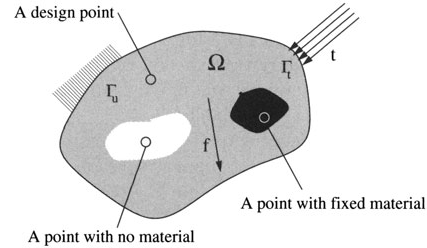
\includegraphics[width=0.6\textwidth]{Pictures/TopOp/design_domain.png}
\caption{The reference domain $\Omega$ for the minimum compliance problem. The problem is formulated such that for a set of external loads $t$ on boundaries $\lambda_t$, body forces $f$ and a set of fixed support points $\lambda_u$, the material distribution within $\Omega$ is such that the stiffness with regards to these loads and forces is maximal and the energy stored by the application of those forces is minimal. The problem also allows defining areas which either cannot or must be filled with material. Figure from \cite{bendsoe2003topology}.}
\label{fig:topOpRefDomain}
\end{figure}
In order to constrain the resulting structure as little as possible, the formulation of the topology optimization problem is generally given as follows: for a given set of external fixture points, external loads and/or body forces, the distribution of material within the reference domain should be found such that the structure has maximum stiffness. This is obtained when the structure has the minimum energy stored by external work for the applied forces. The problem is also usually formed to allow for regions in the domain to be specified as filled or empty of material (see \autoref{fig:topOpRefDomain}). 

The formulation allows the problem to be cast as finding a displacement field $u$ and a stiffness tensor field $E$ that is in equilibrium with the applied loads, and that minimizes the external work done by these external loads do to reach that equilibrium. 

\subsection{Physical and Mathematical Simplifications}
To turn this into a more tractable mathematical problem, a few physical assumptions are also typically made: the material be isotropic and linearly elastic. From the assumptions of isotropy and linear elasticity of the material, the stiffness field becomes a constant of the material, defined where there is material in the domain.

The problem is also easy to cast into a weak form. First of all, we compute the integrated internal virtual work and external work. The former is the work of deforming the elastic material from equilibrium by an admissible displacement. The latter is done by the loads and forces to bring out this displacement. Having computed these, we set them equal to one another in order to conserve energy. As a result we obtain an equation that relates the equilibrium displacement, stiffness tensor, and the forces and loads. We then cast this into the weak form, which can be solved using Finite Element Methods (FEM). These can also incorporate the calculation of the external work done.

\subsection{Solid Isotropic Material with Penalization (SIMP)}
As described in the previous section, we aim to minimise the external work done by looking at different material distributions. However, the usual problem of finding an optimum arises: the search space is vast. After discretising the domain with FEM, the possibilities of where to put material at least are not infinite --- but they still grow exponentially with the number of elements; hence, trying out one-by-one is not going to prove efficient. One popular way of recasting the problem to allow for easier solving is the SIMP model. Here, instead of either being present or not at a point, the material presence can take a continuous set of values between one and zero. The total final volume is then obtained and fixed by integrating this presence variable over the domain, instead of constraining the allowed occupied space. This allows for the interpretation as some kind of density.

In order to still obtain topologies where material is predominant in certain areas --- of densities one, with the rest being empty at densities close to zero --- a "penalty" is applied to the intermediate values. This is effected by raising the density to a power $> 1$ in the elastic energy calculation, but not in the volume calculation. That way, an intermediate density value provides less elastic support, but still "costs" as much volume, and will thus be suboptimal. 

\subsection{Solution and Implementation}
\begin{figure}
\centering
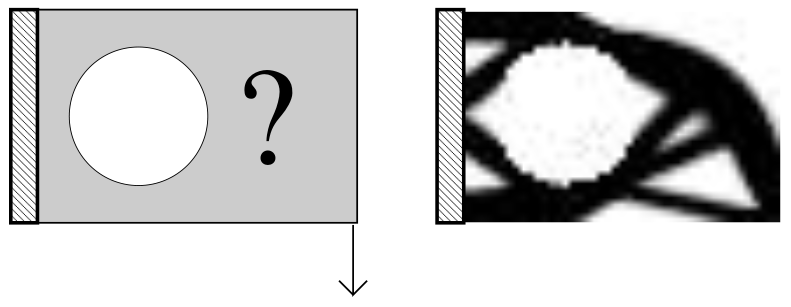
\includegraphics[width=0.6\textwidth]{Pictures/TopOp/Sigmund_cantilever2d.png}
\caption{Topology optimisation of end-loaded cantilever with fixed hole. The optimisation of a loaded cantilever is one of the model problems in topology optimisation, due to its simplicity and its multitude of used solutions throughout the history of engineering. The picture is taken from a known paper by Sigmund \cite{sigmund200199} where a 99-line Matlab code for topology optimisation is introduced.} 
\label{fig:sigmundcantilever}
\end{figure}
In typical implementations, a heuristic iterative scheme is then used for finding a solution. The optimal solution is assumed to have all present parts stressed (as they would otherwise be unnecessary, not providing any support). Thus, at places where the elastic energy is high, material is added if possible, and where it is low, material is likewise removed, with the values "high" and "low" being determined dynamically to keep the total volume constraint. 

This whole scheme is one of the simpler topology optimisation schemes to implement, and has been done so in several pieces of open-source software, including a known 99-line Matlab code by Sigmund \cite{sigmund200199} and ToPy described in \autoref{sec:ToPy}. An example optimised topology is shown in \autoref{fig:sigmundcantilever}. For an extended explanation and discussion, as well as further alternative methods for topology optimisation, the interested reader is referred to \cite{bendsoe2003topology}.

